\apendice{Documentación de usuario}

\section{Introducción}
En este apartado se van a explicar los requisitos que necesita el usuario para poder utilizar el software realizado durante el proyecto, además de una guía detallada de las funciones que puede realizar.

\section{Requisitos de usuarios}
El usuario va a necesitar diferentes requisitos para poder utilizar las aplicaciones del proyecto:

\begin{itemize}
    \item El usuario necesita un navegador moderno capaz de soportar elementos como HTML5 utilizados en el proyecto.
    \item Si se pretende ejecutar en un contenedor docker es necesario tener instalado docker desktop.
    \item Se necesita conexión a internet  para poder disfrutar correctamente de la aplicación web, ademas de para poder ejecutar el proyecto en un contenedor docker. 
    \item Si el usuario pretende crear sus propios archivos csv de forma manual para cargarlos en la aplicación puede utilizar un editor de código.
\end{itemize}



\section{Instalación}

\subsection{Ejecución en local}
Para poder ejecutar correctamente las aplicaciones web en modo local se recomienda al usuario seguir los pasos especificados en el apartado:\hyperref[ejec_local]{Ejecución en local} referente a la documentación del manual del programador.

\subsection{Ejecución en Docker}
Para poder ejecutar correctamente el proyecto en un contenedor docker se recomienda al usuario seguir los pasos especificados en el apartado:\hyperref[ejec_docker]{Ejecución en Docker} referente a la documentación del manual del programador.

\section{Manual del usuario}
En este apartado se van a explicar en detalle todas las funcionalidades de las que puede disponer el usuario al ejecutar el proyecto. Como el proyecto se compone de dos aplicaciones web se explicaran por separado.


\subsection{webhook\_flask}

Suponiendo que se hayan seguido de forma correcta todos los pasos indicados anteriormente sobre la instalación y ejecución del proyecto, si iniciamos la aplicación webhook\_flask la terminal debería verse así:

\begin{figure}[h]
    \centering
    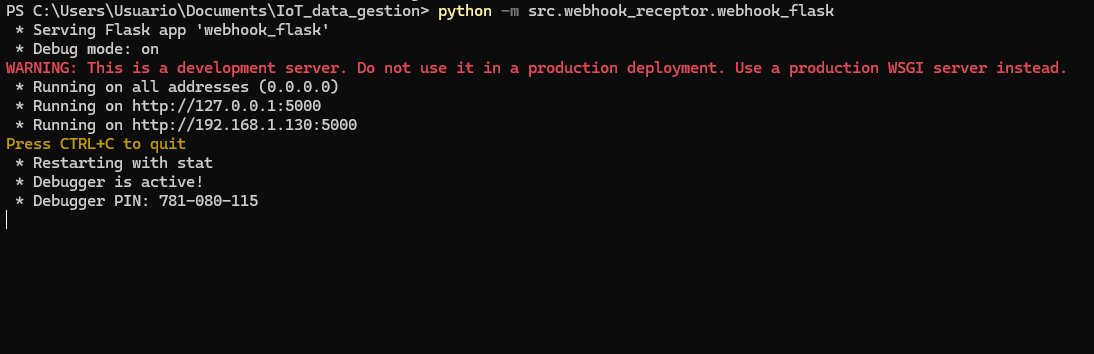
\includegraphics[width=0.8\textwidth]{img/webhook_flask.png} 
    \caption{Imagen de la correcta ejecución de webhook\_flask}
    \label{fig:E1}
\end{figure}

Como se muestra en la imagen, la aplicación actualmente se encuentra ejecutándose en el puerto local 5000. En esta terminal se irán mostrando mensajes referentes a cómo va interactuando la aplicación, ya sea recibiendo, analizando o almacenando paquetes:


\begin{figure}[h]
    \centering
    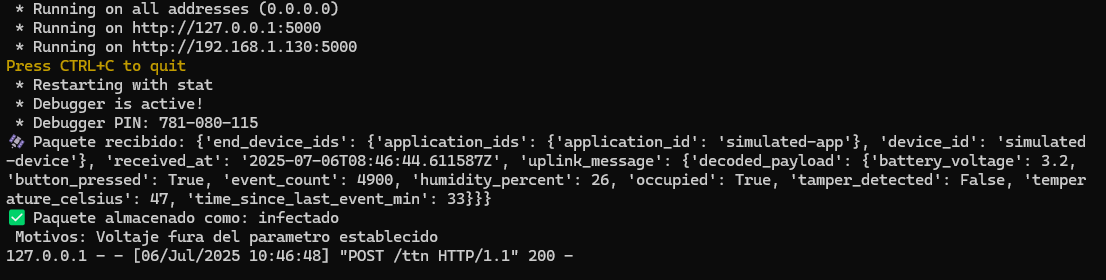
\includegraphics[width=1.2\textwidth]{img/paquete_recibido.png} 
    \caption{Imagen de la aplicación recibiendo correctamente un paquete}
    \label{fig:E2}
\end{figure}

En esta imagen se observa que el paquete ha sido recibido correctamente, se muestra el contenido del mismo, además de notificar qué estado se ha otorgado a ese paquete y el motivo por el cual se le ha otorgado dicho estado. 

\subsection{dashboard\_flask}
Suponiendo que se hayan seguido de forma correcta todos los pasos indicados anteriormente sobre la instalación y ejecución del proyecto, si iniciamos la aplicación dashboard\_flask deberíamos poder acceder a ella a través de esta dirección:

\href{http://localhost:5001/}{http://localhost:50001/}


\subsubsection{Inicio de sesión}
Lo primero que el usuario visualiza en la aplicación es una pestaña de login securizada que no le permite acceder a ninguna funcionalidad de la aplicación hasta que se registre e inicie sesión. Si el usuario no desea crearse una cuenta personal, puede iniciar sesión con:

nombre de usuario: admin

contraseña: admin

La siguiente imagen muestra la pestaña referente al login donde el usuario debe introducir un usuario y contraseña registrados en la base de datos para poder acceder a la aplicación.

\imagen{dh_login.png}{Pestaña de login}

La siguiente imagen muestra la pestaña referente al registro donde el usuario debe introducir un usuario no registrado y una nueva contraseña para poder registrar las credenciales en la base de datos y poder iniciar sesión en el futuro.

\imagen{dh_registro.png}{Pestaña de registro}

La siguiente imagen muestra la pestaña referente a recuperar contraseña donde el usuario debe introducir el nombre de  usuario del que desea restablecer la contraseña, un archivo csv personal que se encuentre en su carpeta de almacenamiento, para asegurar que realmente la contraseña que desea restablecer pertenece a su cuenta  y una nueva contraseña para poder iniciar sesión en la cuenta con la contraseña olvidada.

\imagen{dh_recuperar.png}{Pestaña de recuperar contraseña}

Para visualizar mejor el funcionamiento de estas pestañas, se recomienda al usuario consultar el Vídeo Login:

\href{https://github.com/VictorDeMarco/IoT_data_gestion/tree/main/docs/videos}{https://github.com/VictorDeMarco/IoT\_data\_gestion/tree/main/docs/videos}.

\subsubsection{Visualizar gráficas}
Una vez iniciada sesión lo primero que ve el usuario son las gráficas correspondientes al fichero base (webhook\_dataset):


\imagen{dh_grafica.png}{Pestaña de visualizar las gráficas}

En esta imagen ya se empieza a observar la estructura de la aplicación web, con una barra lateral común a todas las pestañas que permite navegar por la aplicación.

En esta pestaña el usuario puede interactuar con las gráficas eligiendo qué modo desea ver de las mismas (solo reales, solo infectados y todos los datos), pulsando en el desplegable \textbf{Modo de visualización}. 

Además, al pasar con el ratón por encima de la gráfica, puede observar el valor de cada punto y el paquete al que pertenece.

A continuación, se explicará el funcionamiento de la barra lateral. Al ser común a todas las pestañas de la aplicación, lo descrito a continuación se aplica a toda la interfaz.

\begin{itemize}
    \item Se puede observar debajo de TFG el nombre de usuario que esta utilizando la aplicación actualmente.
    \item Si se pulsa el botón \textbf{Dashboard} te redirige a la pestaña de visualización de gráficas.
    \item Si se pulsa el botón \textbf{Ficheros CSV} te redirige a la pestaña de listado de ficheros.
    \item Si se pulsa el botón \textbf{Infectar} te redirige a la pestaña de simulación de envió de paquetes a la aplicación webhook .
    \item Si se pulsa el botón \textbf{Cerrar sesión} te redirige a la pestaña de inicio de sesión, obligándote a volver a iniciar sesión si deseas continuar usando la aplicación.
\end{itemize}

Para visualizar mejor el funcionamiento de la visualización de gráficas, se recomienda al usuario consultar el Vídeo Gráficas:

\href{https://github.com/VictorDeMarco/IoT_data_gestion/tree/main/docs/videos}{https://github.com/VictorDeMarco/IoT\_data\_gestion/tree/main/docs/videos}.

\subsubsection{Ficheros csv}
Como se ha mencionado anteriormente, si pulsas el botón \textbf{Ficheros CSV}  en la barra lateral, llegas a esta pestaña, donde se muestra el listado de ficheros csv almacenados en el proyecto, con los cuales puedes:

\begin{itemize}
    \item Visualizar su contenido.
    \item Aplicar su contenido para visualizarlo en las gráficas de la pestaña Dashboard.
    \item Eliminar el fichero.
    \item Descargar el fichero.
\end{itemize}

\imagen{dh_csv.png}{Pestaña con la lista de ficheros}

En esta imagen se muestra la pestaña con la lista de ficheros disponibles en el proyecto, en este ejemplo solo se dispone del archivo base. Además de las funciones mencionadas en la gestión de archivos, en esta pestaña hay dos funciones más relacionadas con el subir nuevos ficheros csv al proyecto.

La primera de ellas es Añadir fichero:

\imagen{dh_añadir.png}{Pestaña para añadir un nuevo fichero}

Después de que en la pestaña con la lista de ficheros el usuario pulse el botón añadir fichero, se le redirige a esta pestaña, donde puede elegir entre arrastrar un archivo desde su dispositivo a la web o pulsar el botón seleccionar archivo, el cual le mostrará los archivos csv que se encuentran en su dispositivo, para que seleccione uno que quiera añadir a la lista.

Después de que el programa analice si el contenido del archivo es compatible con la aplicación, lo añade a la lista personal del usuario o notifica al usuario el error por el cual no se ha podido añadir.


La segunda de ellas es Analizar fichero:

\imagen{dh_analizar.png}{Pestaña para analizar un fichero}

Después de que en la pestaña con la lista de ficheros el usuario pulse el botón analizar fichero, se le redirige a esta pestaña, donde puede elegir entre arrastrar un archivo desde su dispositivo a la web o pulsar el botón seleccionar archivo, el cual le mostrará los archivos csv que se encuentran en su dispositivo, para que seleccione uno que quiera añadir a la lista.

El programa comprueba que el contenido del archivo csv sea válido y después hace uso de la función analizar de la aplicación webhook para determinar el valor del atributo estado de cada fila del fichero csv a analizar.

Una vez analizado correctamente el archivo, lo añade a la lista personal del usuario con el sufijo \_analizado.

Para visualizar mejor el funcionamiento de la gestión de archivos csv se recomienda al usuario consultar el Vídeo CSV:

\href{https://github.com/VictorDeMarco/IoT_data_gestion/tree/main/docs/videos}{https://github.com/VictorDeMarco/IoT\_data\_gestion/tree/main/docs/videos}.


\subsubsection{Infectar}
Para acceder a esta función, el usuario debe pulsar el botón infectar, que se encuentra en la barra lateral. Este botón te redirige a la pestaña en la cual se puede simular un envío de paquetes de datos a la aplicación webhook. 

\imagen{dh_infectar.png}{Pestaña para enviar paquetes de datos a la aplicación webhhok}

En esta imagen se muestra que en la pestaña infectar el usuario puede elegir entre dos modos para simular el envió de un paquete de datos, modo manual donde es el usuario el que 
él contenido del paquete a enviar y generar paquete aleatorio para generar un paquete con datos aleatorios.

En el caso del modo manual no se permite dejar al usuario campos vacíos ni introducir letras en los campos, evitando así que el usuario trate de enviar un paquete de datos con datos que la lógica del sistema no es capaz de procesar, pudiendo terminar en la interrupción del proyecto.

Una vez elegido el modo de generación del paquete, antes de ser enviado se le permitirá al usuario la previsualización del contenido para que pueda confirmar si desea enviar ese paquete a la aplicación webhook.

\imagen{dh_paq_ej.png}{Imagen de un ejemplo de paquete preparado para ser enviado}

Para visualizar mejor el funcionamiento de la simulación de envío de paquetes se recomienda al usuario consultar el Vídeo Infectar:

\href{https://github.com/VictorDeMarco/IoT_data_gestion/tree/main/docs/videos}{https://github.com/VictorDeMarco/IoT\_data\_gestion/tree/main/docs/videos}.